\chapter{Wyniki badań}\label{ch:wyniki}

\section{Porównanie reshardingu klastra}

Celem testu było porównanie czasu i wpływu reshardingu na opóźnienia klienta dla trzech wariantów: klasycznej migracji slotów w samodzielnie utrzymywanym klastrze Valkey, atomowej migracji slotów w Valkey oraz zarządzanego klastra Redis w Google Cloud Memorystore. Wariant Memorystore należy interpretować jako pomiar typu black-box, ponieważ użytkownik inicjuje zmianę liczby shardów przez API dostawcy chmurowego, ale nie ma bezpośredniego wglądu w wewnętrzną kolejność przenoszenia slotów, tworzenia lub usuwania węzłów oraz finalnych kontroli stanu.

Dla każdego wariantu wykonano po pięć powtórzeń skalowania z trzech do czterech shardów oraz po pięć powtórzeń skalowania z czterech do trzech shardów. Na rysunkach~\ref{fig:reshard-up-comparison} i~\ref{fig:reshard-down-comparison} przedstawiono rozbicie czasu operacji na widoczne fazy. W przypadku Valkey self-hosted osobno widoczny jest czas skalowania infrastruktury, przenoszenia slotów, usuwania dodatkowych węzłów oraz oczekiwania na stabilny stan klastra. W przypadku Memorystore cały czas operacji jest pokazany jako pojedynczy blok zarządzany przez usługę.

Procedura wykonania testu, kolejność faz oraz parametry obciążenia zostały opisane w podrozdziale~\ref{subsec:resharding}. Poniżej przedstawiono zmierzone czasy operacji oraz wpływ reshardingu na klienta.

\begin{figure}[!htbp]
    \centering
    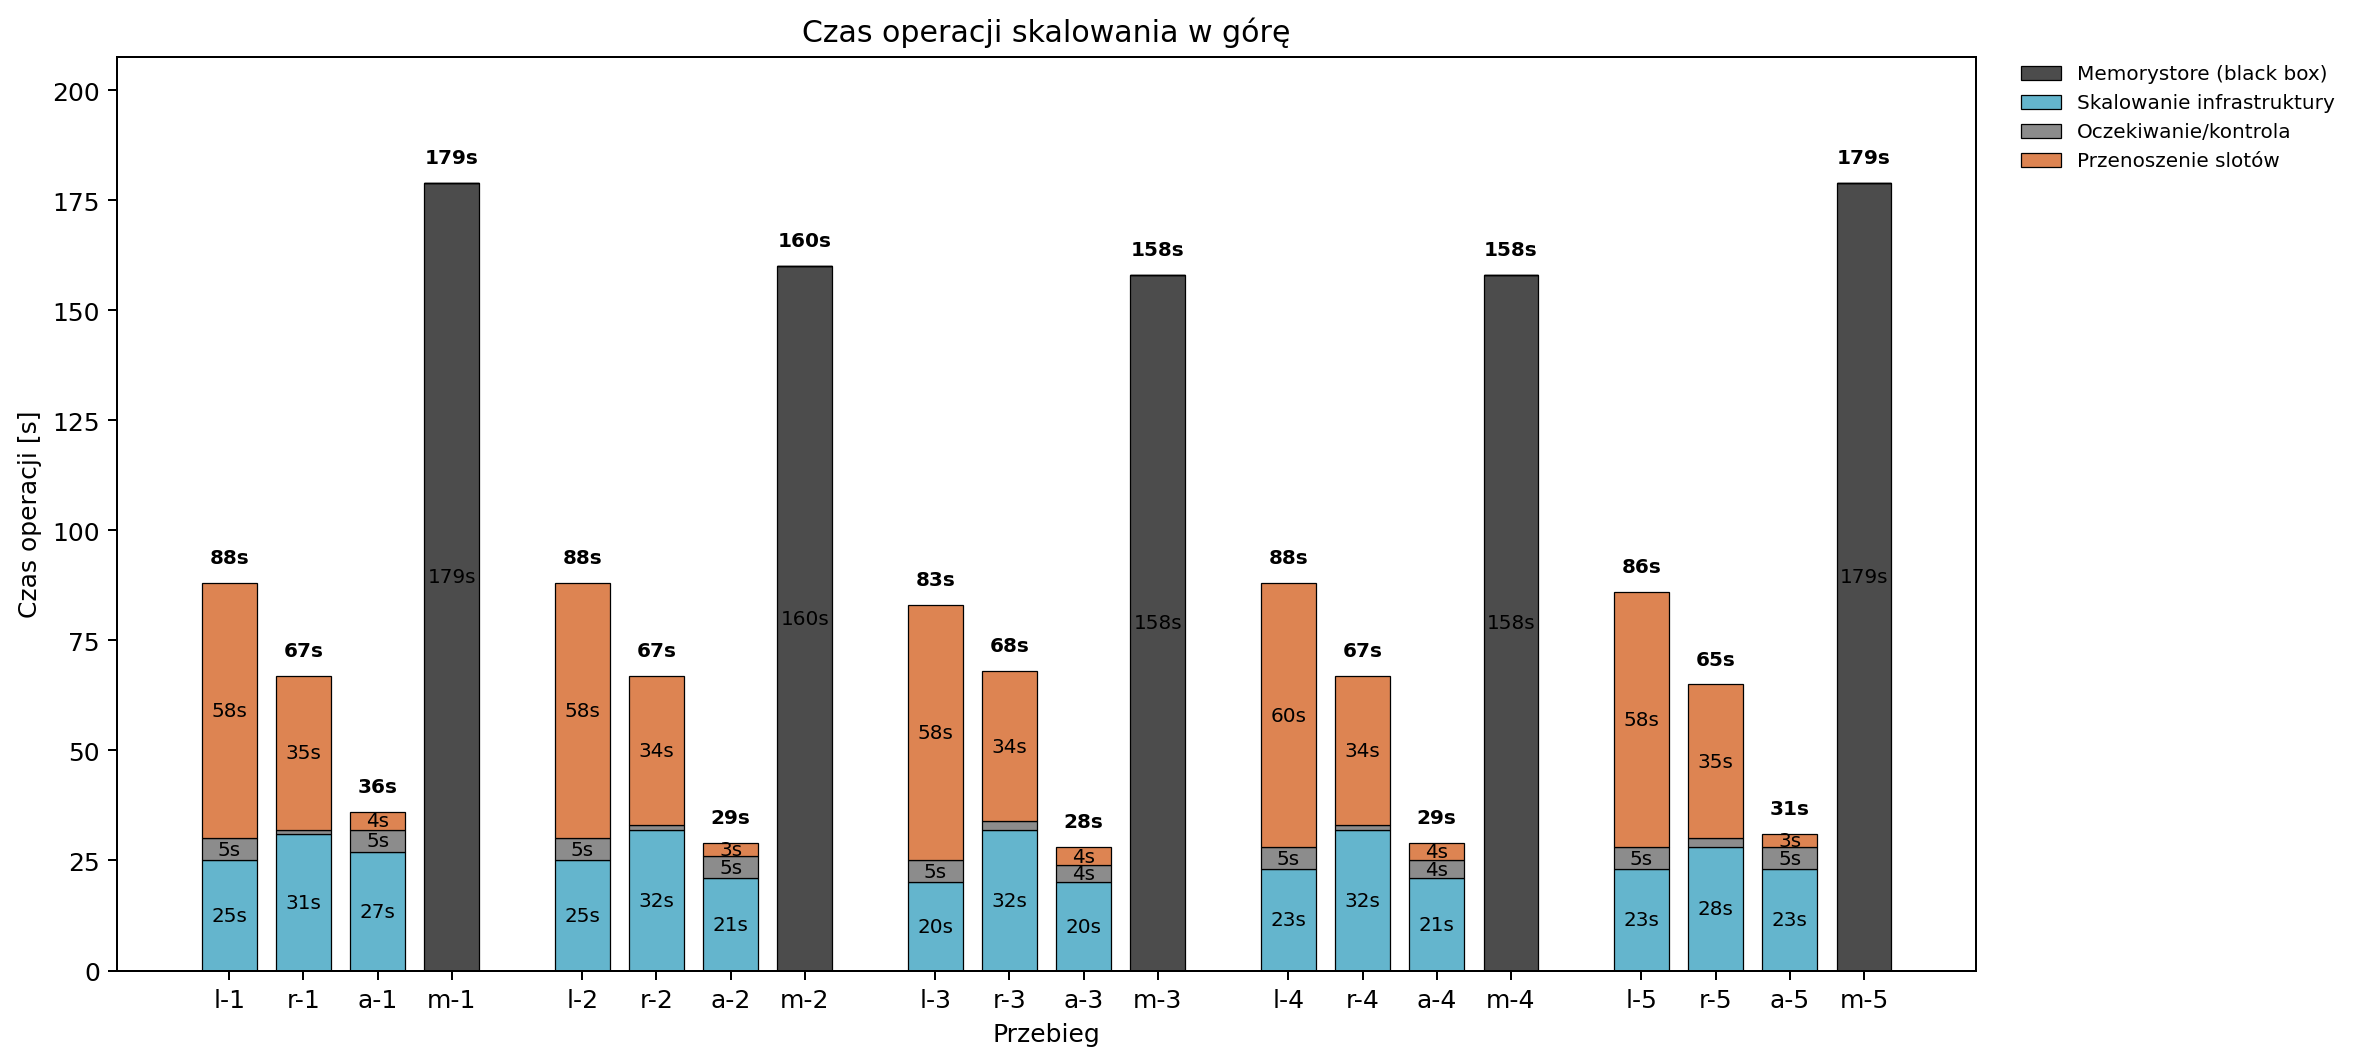
\includegraphics[width=\textwidth]{images/reshard_up_comparison.png}
    \caption{Porównanie czasu skalowania z trzech do czterech shardów dla migracji legacy, migracji atomowej oraz Memorystore.}
    \label{fig:reshard-up-comparison}
\end{figure}

\begin{figure}[!htbp]
    \centering
    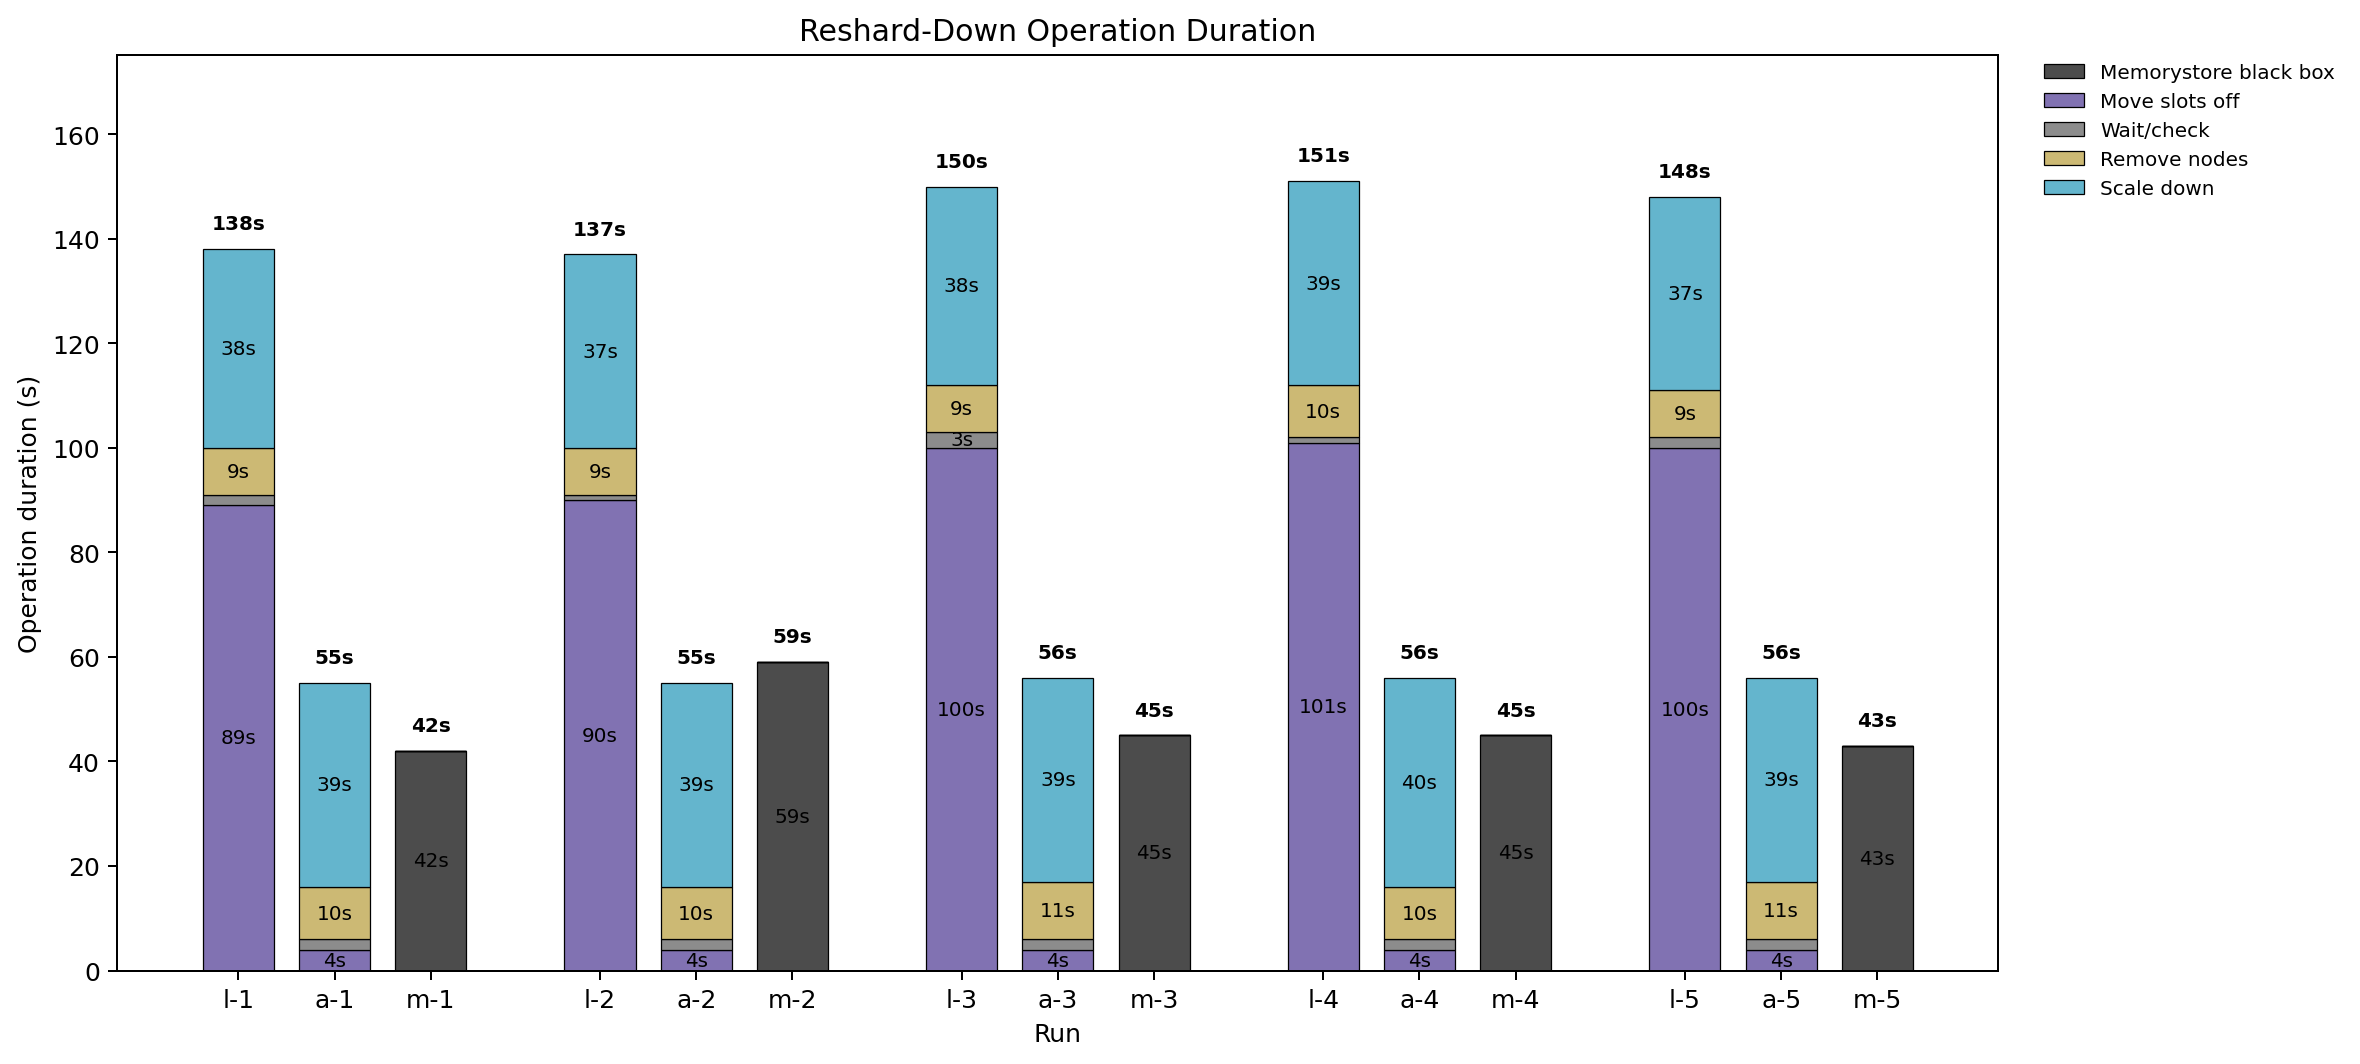
\includegraphics[width=\textwidth]{images/reshard_down_comparison.png}
    \caption{Porównanie czasu skalowania z czterech do trzech shardów dla migracji legacy, migracji atomowej oraz Memorystore.}
    \label{fig:reshard-down-comparison}
\end{figure}

\FloatBarrier

Tabela~\ref{tab:reshard-duration} pokazuje średni czas całej operacji administracyjnej wraz z odchyleniem standardowym. Przyspieszenie zostało policzone względem klasycznej migracji slotów Valkey w tej samej fazie testu.

\begin{table}[htbp]
\centering
\caption{Czas reshardingu i przyspieszenie względem migracji legacy.}
\label{tab:reshard-duration}
\begin{adjustbox}{max width=\textwidth}
\begin{tabular}{lrrrrr}
\toprule
Faza & Legacy [s] & Atomic [s] & Memorystore [s] & Atomic / legacy & Memorystore / legacy \\
\midrule
3 $\rightarrow$ 4 shardy & $103{,}6 \pm 1{,}5$ & $35{,}6 \pm 6{,}6$ & $166{,}8 \pm 11{,}2$ & $2{,}91\times$ & $0{,}62\times$ \\
4 $\rightarrow$ 3 shardy & $144{,}8 \pm 6{,}8$ & $55{,}6 \pm 0{,}5$ & $46{,}8 \pm 6{,}9$ & $2{,}60\times$ & $3{,}09\times$ \\
\bottomrule
\end{tabular}
\end{adjustbox}
\end{table}

\FloatBarrier

Największa różnica między trybem legacy i atomic pojawia się w fazie wykonywanej przez \texttt{valkey-cli --cluster rebalance}. Przy skalowaniu w górę klasyczna migracja zajmowała średnio 76{,}6~s, podczas gdy migracja atomowa 4{,}4~s. Przy skalowaniu w dół różnica była jeszcze bardziej widoczna w części odpowiedzialnej za opróżnienie dodatkowego sharda: 96{,}0~s dla legacy oraz 4{,}0~s dla atomic.

Wynik Memorystore jest asymetryczny. Skalowanie z trzech do czterech shardów trwało średnio 166{,}8~s, czyli dłużej niż oba warianty Valkey self-hosted. Skalowanie z czterech do trzech shardów trwało jednak średnio 46{,}8~s i było szybsze od obu wariantów self-hosted liczonych jako pełna operacja administracyjna.

Wpływ reshardingu na klienta przedstawia tabela~\ref{tab:reshard-latency-throughput}. Wartości percentyli są średnimi z wyników raportowanych przez \texttt{memtier\_benchmark} dla pięciu powtórzeń, natomiast kolumna \textit{ops/sec} zawiera średnią oraz odchylenie standardowe.

\begin{table}[htbp]
\centering
\caption{Przepustowość i percentyle opóźnień podczas reshardingu.}
\label{tab:reshard-latency-throughput}
\begin{adjustbox}{max width=\textwidth}
\begin{tabular}{llrrrrr}
\toprule
Faza & Wariant & Ops/sec & p50 [ms] & p95 [ms] & p99 [ms] & p99.9 [ms] \\
\midrule
3 $\rightarrow$ 4 & Legacy & $105\,999{,}91 \pm 1\,144{,}62$ & 1{,}27 & 6{,}17 & 10{,}97 & 19{,}97 \\
3 $\rightarrow$ 4 & Atomic & $112\,655{,}54 \pm 2\,069{,}61$ & 1{,}28 & 5{,}49 & 10{,}16 & 19{,}53 \\
3 $\rightarrow$ 4 & Memorystore & $141\,327{,}99 \pm 1\,985{,}12$ & 1{,}23 & 2{,}01 & 2{,}95 & 6{,}71 \\
4 $\rightarrow$ 3 & Legacy & $101\,685{,}72 \pm 635{,}51$ & 1{,}62 & 7{,}05 & 11{,}98 & 22{,}07 \\
4 $\rightarrow$ 3 & Atomic & $114\,688{,}15 \pm 2\,664{,}65$ & 1{,}18 & 5{,}24 & 9{,}41 & 18{,}38 \\
4 $\rightarrow$ 3 & Memorystore & $140\,837{,}06 \pm 1\,026{,}09$ & 1{,}47 & 2{,}42 & 3{,}54 & 7{,}45 \\
\bottomrule
\end{tabular}
\end{adjustbox}
\end{table}

\FloatBarrier

Podczas obu faz atomic utrzymał wyższą przepustowość niż legacy oraz niższe opóźnienia w ogonie rozkładu. Dla skalowania w dół p99 spadło z 11{,}98~ms do 9{,}41~ms, a p99.9 z 22{,}07~ms do 18{,}38~ms. Memorystore osiągnął najwyższą przepustowość i najniższe percentyle opóźnień, ale ten wynik należy zestawiać z innym charakterem środowiska: usługa zarządzana działa poza kontrolowanym klastrem Kubernetes i ukrywa część mechanizmów administracyjnych. Z punktu widzenia testu self-hosted najważniejszy wniosek jest taki, że atomowa migracja slotów znacząco skraca okno reshardingu i jednocześnie ogranicza degradację opóźnień względem klasycznej migracji.

\section{Rolling upgrade klastra Valkey}

Celem testu rolling upgrade było sprawdzenie, jak klaster Valkey zachowuje się podczas aktualizacji wersji wykonywanej pod obciążeniem. Procedura testu, parametry \texttt{memtier\_benchmark} oraz sposób działania klienta kontrolnego zostały opisane w podrozdziale~\ref{subsec:rolling_upgrade}. Wyniki dla pięciu powtórzeń przedstawiono w tabeli~\ref{tab:upgrade-results}.

\begin{table}[htbp]
\centering
\caption{Wyniki testu rolling upgrade z perspektywy klienta kontrolnego.}
\label{tab:upgrade-results}
\begin{adjustbox}{max width=\textwidth}
\begin{tabular}{rrrrrrr}
\toprule
Przebieg & Czas [s] & Próby & Błędy & Timeouty & Error rate [\%] & p99 [ms] \\
\midrule
1 & 281 & 1153 & 16 & 11 & 1{,}39 & 111{,}44 \\
2 & 290 & 1202 & 15 & 10 & 1{,}25 & 39{,}99 \\
3 & 268 & 1136 & 15 & 6 & 1{,}32 & 40{,}95 \\
4 & 282 & 1205 & 13 & 6 & 1{,}08 & 35{,}96 \\
5 & 269 & 1136 & 16 & 7 & 1{,}41 & 34{,}65 \\
\midrule
Śr. $\pm$ odch. std. & $278{,}0 \pm 9{,}35$ & $1166{,}4 \pm 34{,}6$ & $15{,}0 \pm 1{,}22$ & $8{,}0 \pm 2{,}35$ & $1{,}29 \pm 0{,}13$ & $52{,}60 \pm 33{,}00$ \\
\bottomrule
\end{tabular}
\end{adjustbox}
\end{table}

\FloatBarrier

Średni czas rolling upgrade wyniósł 278~s. W oknie aktualizacji klient kontrolny zarejestrował średnio 15 błędów na około 1166 prób, co odpowiada 1{,}29\% nieudanych operacji. Najczęściej były to timeouty operacji \texttt{SET}; pojawiały się również odpowiedzi \texttt{CLUSTERDOWN} oraz pojedyncze błędy połączenia. Podczas rozruchu oraz po zakończeniu aktualizacji nie zarejestrowano błędów.

\section{Backup i restore}

Celem testu było porównanie czasu wykonania kopii zapasowej i odtworzenia klastra dla dwóch wariantów: samodzielnie utrzymywanego klastra Valkey w Kubernetes z backupem opartym o snapshoty GCE Persistent Disk oraz zarządzanego klastra Redis w Google Cloud Memorystore z wbudowanym mechanizmem backupu. Procedura testu, fazy operacji oraz sposób weryfikacji integralności zostały opisane w podrozdziale~\ref{subsec:backup_restore}. Dla każdego wariantu wykonano po pięć powtórzeń na zbiorze danych o rozmiarze 10\,240~MB (10\,485\,760 kluczy).

\subsection{Valkey self-hosted --- PVC snapshots}

Tabela~\ref{tab:backup-valkey-phases} przedstawia średni czas poszczególnych faz backupu i odtworzenia wraz z odchyleniem standardowym. Rozbicie na fazy pokazano na rysunku~\ref{fig:valkey-backup-breakdown}.

\begin{table}[htbp]
\centering
\caption{Czas poszczególnych faz backupu i restore dla klastra Valkey (5 powtórzeń, 10~GB danych).}
\label{tab:backup-valkey-phases}
\begin{adjustbox}{max width=\textwidth}
\begin{tabular}{lrr}
\toprule
Faza & Średni czas [s] & Odch. std. [s] \\
\midrule
\multicolumn{3}{l}{\textit{Backup}} \\
\quad BGSAVE & $12{,}2$ & $0{,}84$ \\
\quad Skalowanie StatefulSet do 0 & $33{,}2$ & $0{,}84$ \\
\quad Tworzenie snapshotów dysków & $220{,}2$ & $5{,}63$ \\
\quad \textbf{Łączny czas backupu} & $\mathbf{266{,}0}$ & $\mathbf{5{,}39}$ \\
\midrule
\multicolumn{3}{l}{\textit{Restore}} \\
\quad Tworzenie dysków ze snapshotów & $133{,}0$ & $0{,}00$ \\
\quad Tworzenie PV/PVC & $9{,}8$ & $3{,}70$ \\
\quad Uruchomienie podów & $22{,}0$ & $0{,}71$ \\
\quad Odzyskanie stanu klastra & $3{,}0$ & $2{,}74$ \\
\quad \textbf{Łączny czas restore} & $\mathbf{169{,}8}$ & $\mathbf{5{,}02}$ \\
\midrule
Weryfikacja integralności (10\% próbka) & $256{,}2$ & $10{,}47$ \\
\bottomrule
\end{tabular}
\end{adjustbox}
\end{table}

\begin{figure}[!htbp]
    \centering
    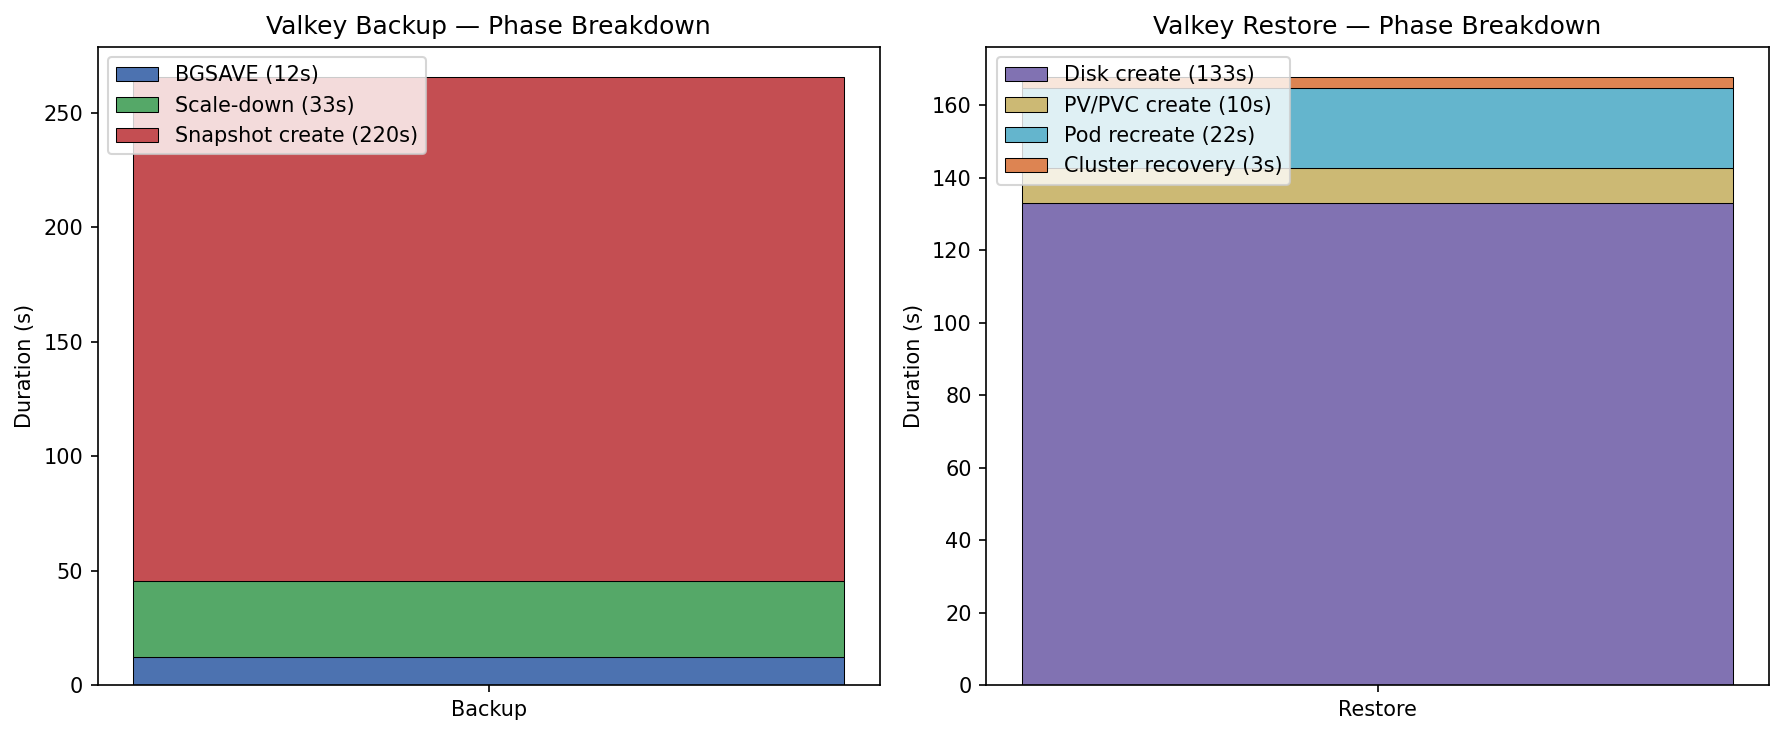
\includegraphics[width=\textwidth]{images/valkey_backup_phase_breakdown.png}
    \caption{Rozbicie czasu backupu i restore klastra Valkey na poszczególne fazy.}
    \label{fig:valkey-backup-breakdown}
\end{figure}

\FloatBarrier

Dominującą fazą backupu jest tworzenie snapshotów dysków GCE (średnio 220{,}2~s, co stanowi 83\% całkowitego czasu backupu). Sam zapis RDB trwał jedynie 12{,}2~s. Po stronie odtworzenia najdłuższą operacją jest tworzenie dysków ze snapshotów (133{,}0~s, 78\% czasu restore). Czas uruchomienia podów i osiągnięcia gotowości klastra wyniósł łącznie 25~s.

Integralność danych została potwierdzona w 4 z 5 przebiegów. W przebiegu numer 4 weryfikator zgłosił 3 błędy na próbce 1\,048\,576 kluczy (0{,}0003\%), przy zerowej liczbie brakujących kluczy. Ponieważ żadne klucze nie zostały utracone, błędy te mogą wynikać z różnicy w momencie wykonania BGSAVE na poszczególnych shardach.

\subsection{Memorystore --- zarządzany backup}

Tabela~\ref{tab:backup-memorystore} przedstawia wyniki dla usługi Memorystore.

\begin{table}[htbp]
\centering
\caption{Czas backupu i restore dla Memorystore (5 powtórzeń, 10~GB danych).}
\label{tab:backup-memorystore}
\begin{adjustbox}{max width=\textwidth}
\begin{tabular}{lrr}
\toprule
Faza & Średni czas [s] & Odch. std. [s] \\
\midrule
Backup (zarządzany) & $49{,}4$ & $8{,}14$ \\
Restore (utworzenie klastra z backupu) & $475{,}4$ & $17{,}90$ \\
Weryfikacja integralności & $470{,}4$ & $8{,}93$ \\
\bottomrule
\end{tabular}
\end{adjustbox}
\end{table}

\FloatBarrier

Backup zarządzany trwał średnio 49{,}4~s, co jest ponad pięciokrotnie szybsze od wariantu self-hosted (266{,}0~s). Wynika to z faktu, że Memorystore nie wymaga zatrzymania klastra ani tworzenia snapshotów wolumenów --- usługa wykonuje kopię wewnętrznie. Natomiast operacja odtworzenia (utworzenie nowego klastra z backupu) trwała średnio 475{,}4~s, czyli prawie trzykrotnie dłużej niż restore w wariancie self-hosted (169{,}8~s). Wynika to z konieczności alokacji i konfiguracji nowej infrastruktury klastra przez dostawcę chmurowego. Integralność danych została potwierdzona we wszystkich pięciu przebiegach.

\subsection{Porównanie wariantów}

Rysunek~\ref{fig:backup-comparison} zestawia czasy backupu i restore obu wariantów. Tabela~\ref{tab:backup-comparison-total} podsumowuje łączny czas operacji.

\begin{figure}[!htbp]
    \centering
    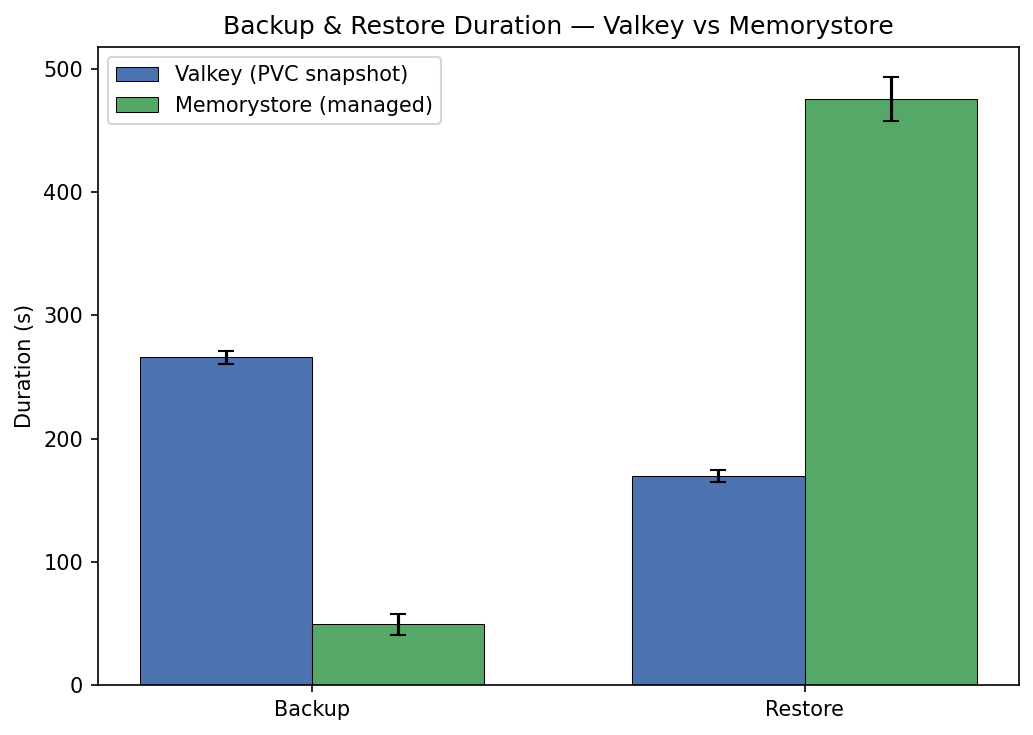
\includegraphics[width=0.85\textwidth]{images/backup_comparison.png}
    \caption{Porównanie czasu backupu i restore między Valkey self-hosted a Memorystore.}
    \label{fig:backup-comparison}
\end{figure}

\begin{table}[htbp]
\centering
\caption{Porównanie łącznego czasu backupu i restore.}
\label{tab:backup-comparison-total}
\begin{adjustbox}{max width=\textwidth}
\begin{tabular}{lrrr}
\toprule
Operacja & Valkey [s] & Memorystore [s] & Stosunek \\
\midrule
Backup & $266{,}0 \pm 5{,}4$ & $49{,}4 \pm 8{,}1$ & $5{,}38\times$ \\
Restore & $169{,}8 \pm 5{,}0$ & $475{,}4 \pm 17{,}9$ & $0{,}36\times$ \\
Łącznie (backup + restore) & $435{,}8$ & $524{,}8$ & $0{,}83\times$ \\
\bottomrule
\end{tabular}
\end{adjustbox}
\end{table}

\FloatBarrier

Warianty prezentują odwrócone proporcje: Memorystore oferuje szybki backup (5{,}4$\times$ krótszy), ale wolny restore (2{,}8$\times$ dłuższy). Łączny czas cyklu backup--restore jest w wariancie self-hosted krótszy o~17\% (435{,}8~s vs 524{,}8~s). Kluczowa różnica operacyjna polega na tym, że backup Valkey wymaga niedostępności klastra na czas skalowania w dół i tworzenia snapshotów (łącznie ${\sim}253$~s), natomiast backup Memorystore nie powoduje przestoju w obsłudze zapytań.
